\documentclass[../xdudla00-porting-Tang-to-Open-WRT.tex]{subfiles}
\begin{document}

\chapter{Encryption}\label{encryption}


We may not realize this, but we use encryption every day.
The purpose of encryption itself is to keep us safe when we are browsing the internet or just storing our sensitive information on digital media. 
In general encryption is used to secure our data, whether transmitted around the internet or stored on our hard drives, from being compromised.
The encryption protects us from many threats.

It protects us from identity theft. 
Our personal information stored all over governmental authorities are secured with it.
Encryption care for not revealing sensitive information about ourselves, to protect our financial details, passwords and so on. 
Mainly when we bank online from being scammed.

It look after our conversation privacy. 
To be more specific our cell phone conversations from eavesdroppers and our online chatting with acquaintances or colleagues. 
It also allows attorneys to communicate privately with their clients and it aims to secure communication between investigation bureaus to exchange sensitive information about lawbreakers.

If we encrypt our laptop or desktop computer's hard drive it protects our data if it is stolen. 

\section{Hard drive encryption}


Studies show that\dots \todo{PDF}

First, lets take a look on how the encryption is typically done.
It all starts, as mentioned above, with desire to keep our data to ourselves and as a secret to the other people.
More often than not, these secrets are stored on our hard drives.

To protect our secrets we usually encrypt these data, stored on our hard drive, by using an encryption key - see Figure \ref{fig:encdata}.
However, our secret data might grow in size, and it is time and resource consuming to decrypt and encrypt the secret every time encryption key changes or it is compromised.
Because of that, we wrap encrypted data in the key encryption key. 
This is actually what the system prompts from us when booting or simply when it wants to access our hard drive.

\begin{figure}[h]
    \centering
    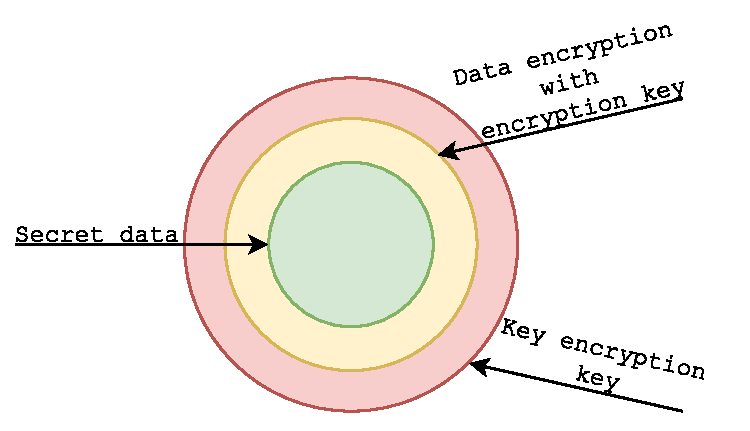
\includegraphics[scale=0.7]{figures/HowWeEncryptData.pdf}
    \caption{How we encrypt data}
    \label{fig:encdata}
\end{figure}

For people is common to have a password protected system.
Imagine you come home in a mood to enjoy your time and your system asks for password, not once, but twice.
This might be the reason why most of us do not use encryption, even when we know it will protect our data.


So, changing the key encryption key does not affect encrypted data.
We can change it whenever we desire to and redistribute the new key to all users or services who are supposed to access these data.

\todo{hmm}This is what Tang \ref{tang} is used for, since we want to automatize things.

To automatize this, we could generate cryptographically stronger key encryption key than user provided password.
Then, we store this cryptographically stronger random key on a remote system, from where we can get it later.
This is basically how the Escrow \ref{escrow} model works.

\subsection{LUKS}
\todo{LUKS HEADER IMAGE}



\end{document}
